\documentclass[12pt,a4paper]{article}
% Языки, которые могут быть использованы.
\usepackage[english,russian]{babel}

% FreeSerif — альтернатива TimesNewRoman
\usepackage{fontspec}
\setmainfont[Ligatures=TeX]{Times New Roman}
\setmonofont[Mapping=,Ligatures=]{Courier New}

% Чтобы сделать буковки ещё красивее.
\usepackage{microtype}

% Картинки, вращение и всё такое. Причём даже в режиме черновика
\usepackage[final]{graphicx}
\usepackage{float}
\usepackage[draft=no]{svg}
\usepackage{pdfpages}

% Чтобы легко менять стиль списков
\usepackage[shortlabels]{enumitem}

\usepackage{unicode-math}
\usepackage{csquotes}
\usepackage{adjustbox}
\usepackage{relsize}

% https://tex.stackexchange.com/questions/14967/source-code-listing-with-frame-around-code
\usepackage{listings}
\lstset{frame=lrbt,xleftmargin=\fboxsep,xrightmargin=-\fboxsep}
\lstset{basicstyle=\ttfamily,breaklines=true}

% https://qna.habr.com/answer?answer_id=1140867
\bibliographystyle{gost2008}
\usepackage[
	style=gost-numeric, % стиль цитирования и библиографии, см. документацию biblatex-gost
	language=auto,  % использовать язык из babel
	autolang=other, % многоязычная библиография
	parentracker=true,
	backend=biber,
	hyperref=true,
	bibencoding=utf8,
	sorting=ntvy,  % сортировка: имя, заголовок, том, год
]{biblatex}
\addbibresource{bibliography.bib}
\DeclareSourcemap{
    \maps{
        \map{% если @online, то устанавливаем media=eresource.
            \step[typesource=online, fieldset=media, fieldvalue=eresource]
        }
    }
}

% Отсупы как по госту.
\usepackage[
	includeheadfoot,
	left=20mm,
	right=10mm,
	top=0mm,
	headheight=25mm,
	footskip=5\baselineskip, % footskip is the distance between the textbody and the baseline of the footer
	bottom=15mm,
]{geometry}

\savegeometry{original}
\geometry{bottom=10mm}
\savegeometry{nofooter}
\loadgeometry{original}

%% Некоторые переменные, которые появляются более одного раза

% Название курсовой. Не забывать проценты в конце строк.
\newcommand{\docTitle}{%
	Сервис для индексирования и просмотра репозиториев%
}

\newcommand{\docTitleEng}{%
	Repository Indexing and Viewing Service%
}

% Год написания курсовой.
\newcommand{\YEAR}{
	\the\year{}
}

% RU — код страны
% 17701729 — код НИУ ВШЭ
% 05.15 — регистрационный номер (https://docs.cntd.ru/document/566085681)
% 		В данном случае, Прикладное ПО / Информационные системы для решения специфических отраслевых задач
% 01 — номер редакции документа
% 33 — код вида документа (https://www.swrit.ru/doc/espd/19.101-77.pdf#page=4)
% 01 — номер документа данного вида
%  1 — номер части документа
\newcommand{\docId}{RU.17701729.03.10-01 12 01-1}


% Footer and header
\usepackage{fancyhdr}
\pagestyle{fancy}
\fancyhf{}
\chead{
	%\bf % Сделать жирненьким
	\thepage\\
	\docId
}
\fancyhead[RO]{%
    % В правый верхний колотитул пихаю номер приложения
    {\ifnum\value{addendum}>0 ПРИЛОЖЕНИЕ \theaddendum \fi}
}
\cfoot{%
	\adjustbox{valign=b}{ % baseline of footer at bottom, so margins are correct
		\begin{tabular}{| l | l | l | l | l |}
			\hline & & & & \\
			\hline Изм. & Лист & № докум. & Подп. & Дата \\
			\hline \docId &  &  &  &  \\
			\hline Инв. № подл. & Подп. и дата & Взам. инв. № & Инв. № дубл. & Подп. и дата № \\
			\hline
		\end{tabular}
	}
}
\fancypagestyle{nofooter}{%
	\fancyfoot{}%
}

\renewcommand{\headrulewidth}{0pt}
\renewcommand{\footrulewidth}{0pt}

% Повернуть на 90 градусов
\newcommand{\rot}[2]{\rotatebox[origin=c]{90}{\enspace\parbox{#1 - 0.5em}{#2}}}

% Повторить #1 раз текст #2: \Repeat{#1}{#2}
\usepackage{expl3}
\ExplSyntaxOn
\cs_new_eq:NN \Repeat \prg_replicate:nn
\ExplSyntaxOff

% Продвинутые таблицы
\usepackage{tabularx}
\usepackage{multirow}
\usepackage{xltabular}
% И сразу делаем чтобы колонки X центрировались по вертикали
\def\tabularxcolumn#1{m{#1}}
\newcolumntype{Y}{>{\centering\arraybackslash}X}

% Подсчет числа страниц
\usepackage{lastpage}

% Расчет всяких размеров
\usepackage{calc}

% Названия разделов по центру (но titlesec конфликтует с hyperref)
\usepackage{titlesec}
\titleformat{\section}
  {\centering\Large\bfseries}
  {\thesection}
  {.5em}
  {\MakeUppercase}
% И с точкой в конце.
\titlelabel{\thetitle.\quad}

% После названия раздела надо делать отступы у абзацев.
\usepackage{indentfirst}

% https://tex.stackexchange.com/a/347803
\usepackage{varwidth}

\newcommand{\placename}{
	\underline{\hspace{4cm}}
}
\newcommand{\placedate}{
	«\underline{\hspace{1em}}» \underline{\hspace{3cm}} \YEAR г.
}

\newcounter{addendum}
\makeatletter
\newcommand{\addendum}[1]{
    \stepcounter{addendum}

	% Приложения есть в оглавлении
	\phantomsection
	\addcontentsline{toc}{section}{Приложение \arabic{addendum}: #1}

	\section*{#1}
	
	% Сбросить все счетчики
	\setcounter{equation}{0}
    \setcounter{figure}{0}
    \setcounter{table}{0}

	% Треш и угар с макросами, чтобы обойти проблемы между titlsec и hyperref
	% Цель: \NR@gettitle{Приложение 1: …}, но нужно **сначала** раскрыть \arabic{addendum}
	\edef\addendumTitle{\noexpand\NR@gettitle{Приложение \arabic{addendum}: #1}}
	\addendumTitle
}
\makeatother

% Ещё больше подсекций
\newcommand{\subsubsubsection}[1]{\paragraph{#1}\mbox{}\\}
\setcounter{secnumdepth}{4}
\setcounter{tocdepth}{4}

% TODOшечки
\usepackage{ifdraft}
\ifdraft{
	% Если \document[draft], то нам нужно место в полях для todo.
	\geometry{left=40mm, right=5mm, marginparwidth=35mm}
	\reversemarginpar  % причём слева они выглядят симпатичнее
	\savegeometry{original}
}{}
\usepackage[obeyDraft,textsize=footnotesize,textwidth=35mm]{todonotes}

% Добавляем гипертекстовое оглавление в PDF
% hyperref должен быть последним
\usepackage[hidelinks]{hyperref}

\begin{document}
	\selectlanguage{russian}

	\newenvironment{LeftTablePage}{%
	\thispagestyle{empty}%
	% Временно уменьшаем отступы.
	\newgeometry{left=5mm, top=25mm, bottom=10mm}%
	% Содержимое слева.
	\noindent\begin{minipage}[b]{20mm}
		\rotatebox{90}{
			\begin{tabular}{| c | c | c | c | c |}
				\hline
				Инв. № подл. & Подп. и дата & Взам. инв. № & Инв. № дубл. & Подп. и дата \\
				\hline
				\docId & & & & \\
				\hline
			\end{tabular}%
		}
	\end{minipage}%
	% Основное содержимое
	\begin{samepage}%
	\begin{minipage}[b][\textheight]{\textwidth}\centering%
}{
	\end{minipage}%
	\end{samepage}
	
	% Теперь можно вернуть отступы как были
	\restoregeometry

	\clearpage
}

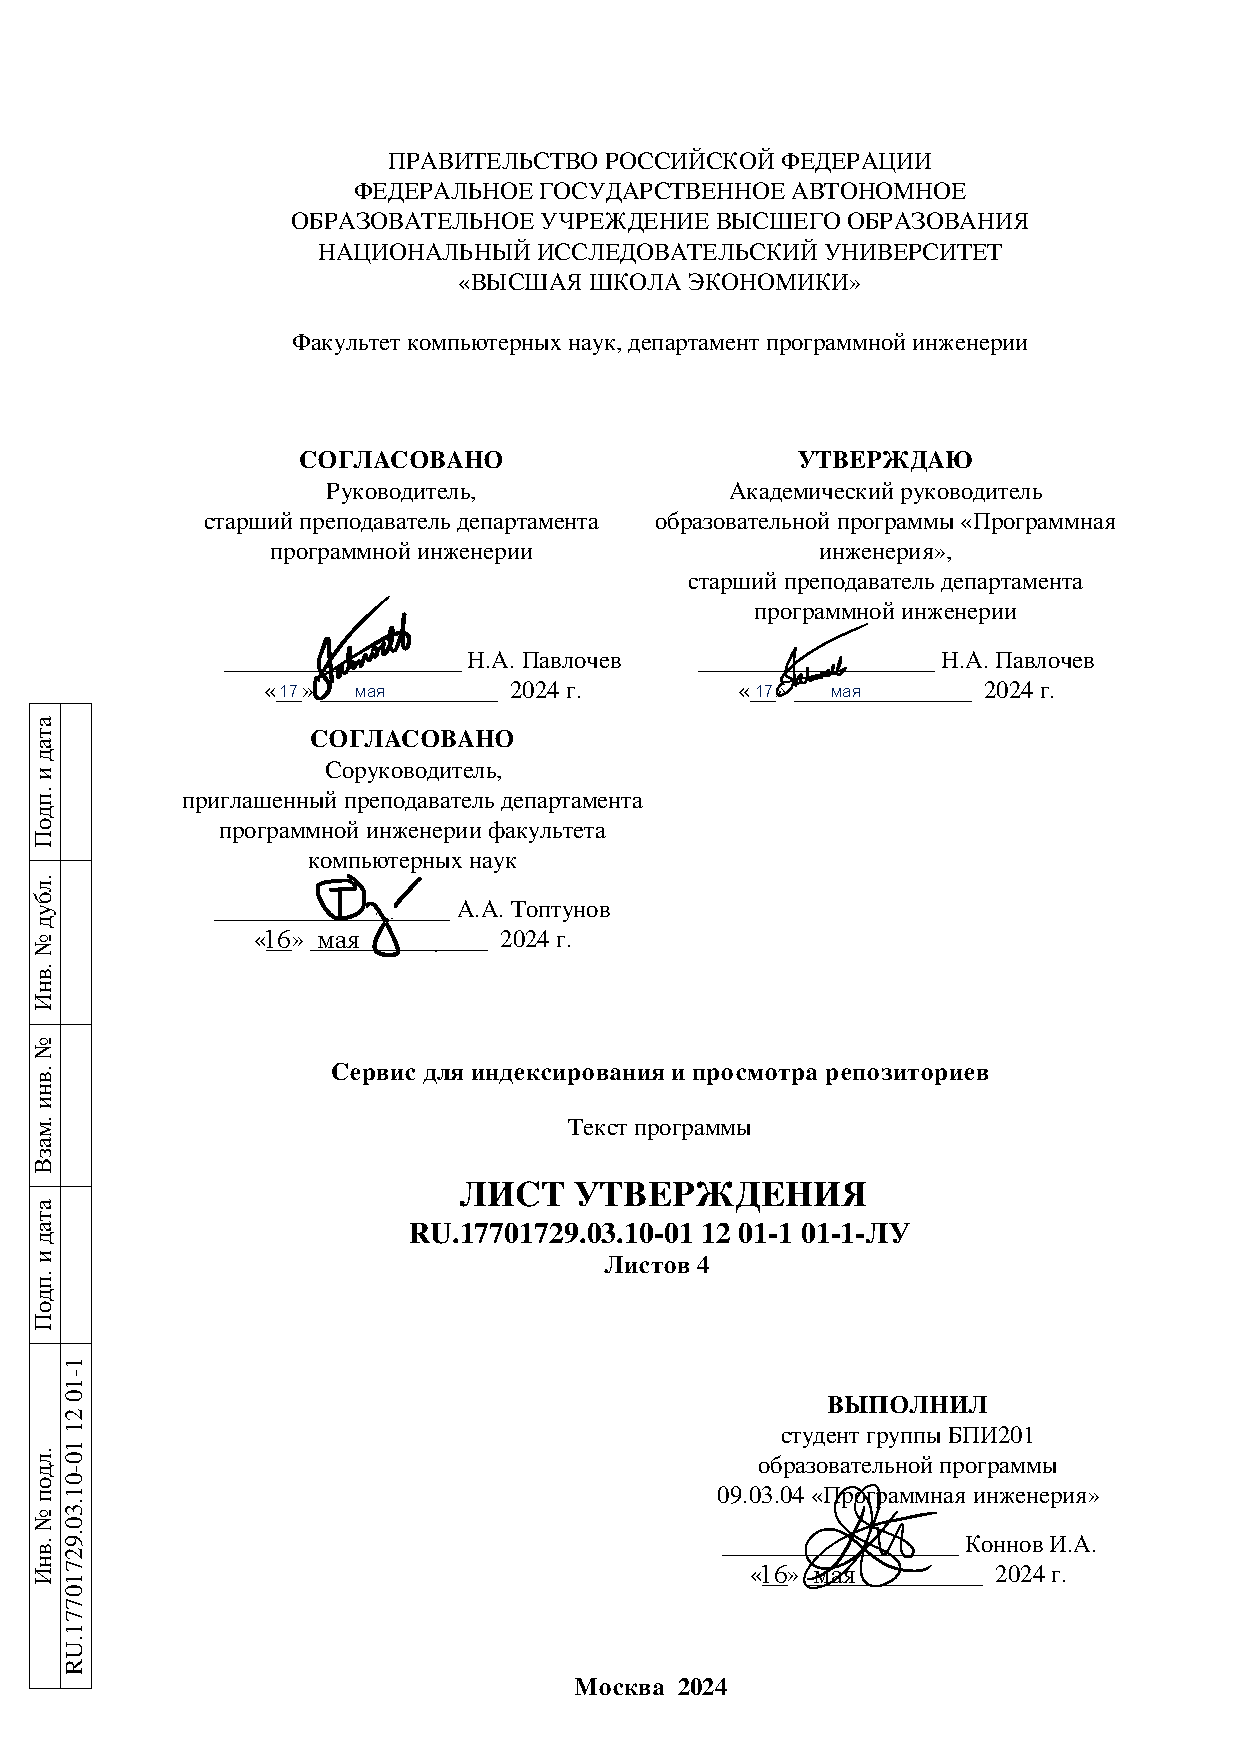
\includepdf[pages=-]{figures/signed.pdf}
% \begin{LeftTablePage}
% 	%% Лист утверждения
    ПРАВИТЕЛЬСТВО РОССИЙСКОЙ ФЕДЕРАЦИИ \\
    ФЕДЕРАЛЬНОЕ ГОСУДАРСТВЕННОЕ АВТОНОМНОЕ \\
    ОБРАЗОВАТЕЛЬНОЕ УЧРЕЖДЕНИЕ ВЫСШЕГО ОБРАЗОВАНИЯ \\
    НАЦИОНАЛЬНЫЙ ИССЛЕДОВАТЕЛЬСКИЙ УНИВЕРСИТЕТ \\
    «ВЫСШАЯ ШКОЛА ЭКОНОМИКИ» \\[1\baselineskip]
    Факультет компьютерных наук, департамент программной инженерии
\vskip 1.5cm
    % Согласовано / утверждаю
    \begin{varwidth}[t]{0.45\textwidth}\centering
    	\textbf{СОГЛАСОВАНО}
    	
    	Руководитель, \\
    	старший преподаватель департамента
        программной инженерии
    \end{varwidth}%
    \hfil%
    \begin{varwidth}[t]{0.45\textwidth}\centering
    	\textbf{УТВЕРЖДАЮ}
    	
    	Академический руководитель
        образовательной программы
        «Программная инженерия», \\
        старший преподаватель департамента
        программной инженерии
    \end{varwidth}

\bigskip

    \begin{varwidth}[t]{0.4\textwidth}\centering
    	\placename Н.А. Павлочев \\
    	\placedate
    \end{varwidth}%
    \hfil%
    \begin{varwidth}[t]{0.4\textwidth}\centering
    	\placename Н.А. Павлочев \\
    	\placedate
    \end{varwidth}

\bigskip

    \begin{minipage}[t]{0.45\textwidth}\centering
    	\textbf{СОГЛАСОВАНО}
    	
    	Соруководитель, \\
    	приглашенный преподаватель
        департамента программной инженерии
        факультета компьютерных наук
    \end{minipage}%
    \hfil\makebox[0.45\textwidth]{}

\bigskip

    \begin{minipage}[t]{0.45\textwidth}\centering
    	\placename А.А. Топтунов \\
    	\placedate
    \end{minipage}%
    \hfil\makebox[0.45\textwidth]{}

\vfill

    \textbf{\uppercase{\docTitle}}

    \bigskip

    Программа и методика испытаний

    \bigskip

    \textbf{
    	\Large
    		ЛИСТ УТВЕРЖДЕНИЯ \\
    	\large
    		{\docId} 01-1-ЛУ \\
    	\normalsize
    		Листов \pageref*{LastPage}
    }

\vfill

    \makebox[0.45\textwidth]{}\hfil%
    \begin{minipage}[t]{0.45\textwidth}\centering
    	\textbf{ВЫПОЛНИЛ}
            
    	студент группы БПИ201 \\
    	образовательной программы \\
    	09.03.04 «Программная инженерия» \\
    \end{minipage}

\bigskip

    \makebox[0.45\textwidth]{}\hfil%
    \begin{minipage}[t]{0.45\textwidth}\centering
    	\placename Коннов И.А. \\
    	\placedate
    \end{minipage}

\vskip 1.5cm

    \textbf{Москва \YEAR}
% \end{LeftTablePage}

% ГОСТ гласит, что лист утверждения не должен быть нумероваться: титульный лист это первый лист
\pagenumbering{arabic}

\begin{LeftTablePage}
	%% Первые две страницы ТЗ:
%% 1. Лист утверждения
%% 2. Титульный лист

\begin{flushleft}
\begin{varwidth}{\linewidth}\centering
	\large
	УТВЕРЖДЕН \\
	{\docId} 01-1-ЛУ
\end{varwidth}
\end{flushleft}

\vskip4cm

{\Large\uppercase{\docTitle}}

\vskip1cm

{\large
	Текст программы

	{\docId} 01-1
}

\vskip1cm

Листов \pageref*{LastPage}

\vfill
\textbf{Москва \YEAR}
\end{LeftTablePage}
	
	
	% На всякий случай, хотя вообще не очень нужно.
	\loadgeometry{original}

	\clearpage
		\renewcommand*\contentsname{\centering СОДЕРЖАНИЕ}
		\tableofcontents
	\clearpage

	% Основное содержимое
	\section{Текст программы}
	Текст программы находится в публичном репозитории на GitHub.
	
	Ссылка на репозиторий: \url{https://github.com/iliakonnov/shatterbird}

	\thispagestyle{nofooter}
\loadgeometry{nofooter}

\section*{ЛИСТ РЕГИСТРАЦИИ ИЗМЕНЕНИЙ}

\noindent\begin{tabularx}{\textwidth}{| p{2ex} | *{9}{X|}}
	\hline 
		\multicolumn{10}{|c|}{Лист регистрации изменений} \\
	\hline
		\multicolumn{5}{|c|}{Номера листов (страниц)}
		& \multirow{2}{\hsize}{Всего листов (страниц в докум.)}
		& \multirow{2}{\hsize}{№ документа}
		& \multirow{2}{\hsize}{Входящий № сопроводительного докум. и дата}
		& \multirow{2}{\hsize}{Подп.}
		& \multirow{2}{\hsize}{Дата} \\
	\cline{1-5}
		\rot{2.5cm}{Изм.}
		& \rot{2.5cm}{Изменённых}
		& \rot{2.5cm}{Заменённых}
		& \rot{2.5cm}{Новых}
		& \rot{2.5cm}{Аннулированных}
		& & & & & \\
	\Repeat{20}{\hline&&&&&&&&&\\[1ex]}
	\hline
\end{tabularx}

\loadgeometry{original}
\clearpage       % Лист регистрации изменений
\end{document}